\documentclass{beamer}
\usepackage{hyperref}
\usepackage{bookmark}
\usepackage{amsmath}
\usepackage[T1]{fontenc}
\usepackage{tabularx}
\usefonttheme[onlymath]{serif}
\usepackage[spanish,provide=*]{babel}
% Cargar apacite después de babel para citas autor-año correctas

% other packages
\usepackage{latexsym,amsmath,xcolor,multicol,booktabs,calligra, tcolorbox}
\usepackage{graphicx,listings,stackengine}
% Manejo robusto de nombres de archivo con espacios y rutas de imágenes
\usepackage{grffile}
%\graphicspath{{pic/}}


\title[Modelamiento de Lahares mediante PINNs]{\large Modelamiento de Lahares mediante Redes Neuronales Informadas por la Física (PINNs): Aplicación
al evento eruptivo de 2015 del volcán Villarica, Chile}

\author[Dylan Jara]{
    \textbf{\small Dylan Jara Carvajal} \\
    \vspace{0.2cm}
    {\scriptsize
    \begin{tabular}{c c c}
        Profesor Guía & Profesor Co-Guía & Profesor Informante \\
        \textbf{Felipe Herrera} & \textbf{Johan Triana} & \textbf{Yuvineza Gomez-Leyton}
    \end{tabular}
    }
}
\institute[DMCC - USACH]{\small
    Departamento de Matemática y Ciencia de la Computación\\
    Universidad de Santiago de Chile
}
\date{\small\today}
\usepackage{./Ritsumeikan}

% defs
\def\cmd#1{\texttt{\color{red}\footnotesize $\backslash$#1}}
\def\env#1{\texttt{\color{blue}\footnotesize #1}}
\definecolor{deepblue}{rgb}{0,0,0.5}
\definecolor{ccnuMainColor}{RGB}{57,64,73}
\definecolor{deepgreen}{rgb}{0,0.5,0}
\definecolor{halfgray}{gray}{0.55}

\lstset{
    basicstyle=\ttfamily\small,
    keywordstyle=\bfseries\color{deepblue},
    emphstyle=\ttfamily\color{ccnuMainColor},    % Custom highlighting style
    stringstyle=\color{deepgreen},
    numbers=left,
    numberstyle=\small\color{halfgray},
    rulesepcolor=\color{red!20!green!20!blue!20},
    frame=shadowbox,
}

\begin{document}

\begin{frame}
    \titlepage
    \vspace*{-0.6cm}
    \begin{figure}
        \begin{center}
                % Ajuste de tamaño más visible y uso de \graphicspath
                
\includegraphics[keepaspectratio, width=0.25\textwidth]{./Pics/Usach S1.png}

        \end{center}
    \end{figure}
\end{frame}

% Restaurar la tabla de contenidos y corregir el problema de 'Referencias32'
\begin{frame}
    \tableofcontents[sectionstyle=show, subsectionstyle=show/shaded/hide]
\end{frame}

%//////////////////////////////////////////////////////%
\section{Introducción}
\subsection{Lahares}
\begin{frame}{Qué son los lahares?}
    \begin{itemize}
        \item Flujos de sedimentos volcánicos que se originan en volcanes potencialmente activos se llaman lahares \cite{Vallance2024}.
    \end{itemize}

        \begin{figure}
        \centering
        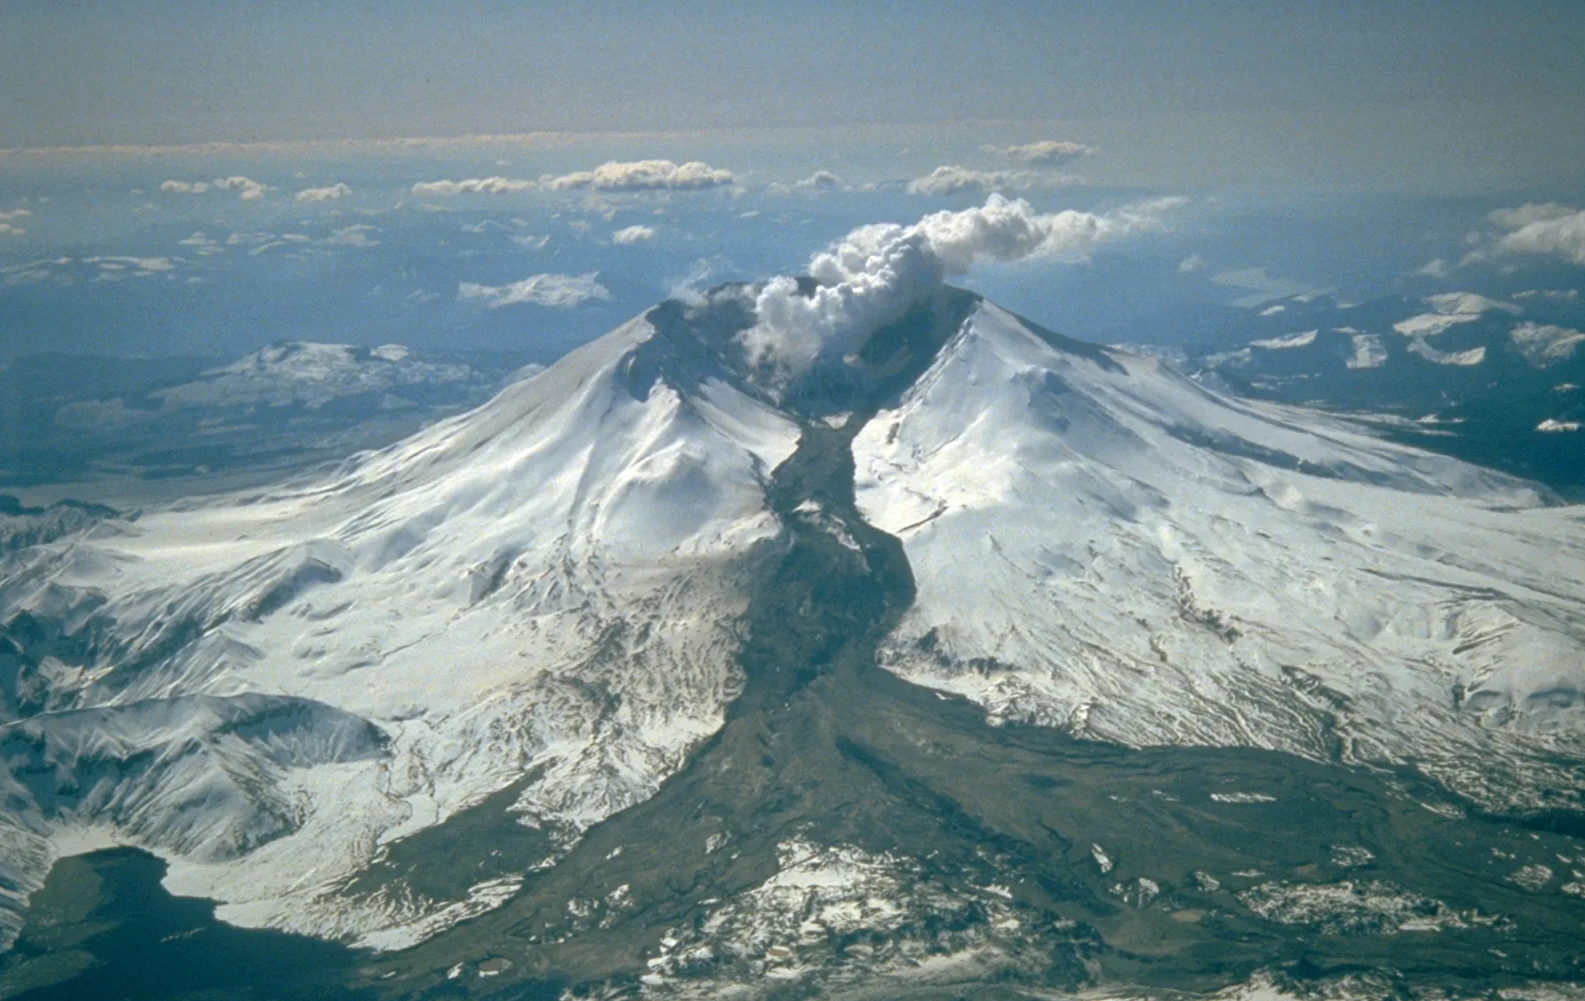
\includegraphics[width=9cm]{.//Pics//lahar.png}
        \caption{Lahar (dark deposit on snow) on Mount Saint Helens after the March 19, 1982, eruption.\cite{article}}
    \end{figure}
\end{frame}


\subsection{Physics-Informed Neural Networks (PINNs)}
\begin{frame}{Qué son las PINNs?}
\begin{itemize}
    \item Las redes neuronales basadas en la física son redes neuronales entrenadas para resolver tareas de aprendizaje supervisado respetando
    cualquier ley física dada descrita por ecuaciones diferenciales parciales no lineales generales \cite{RAISSI2019686}.
    \item $\mathcal{L} = \mathcal{L}_{data} + \lambda \mathcal{L}_{physics}$, donde $\mathcal{L}_{data}$ mide el error en los datos y $\mathcal{L}_{physics}$ mide el incumplimiento de las PDEs.
\end{itemize}
\end{frame}

%/////////////////////////////////////////////%
%/////////////////////////////////////////////%

\section{Objetivo general y motivación}
\begin{frame}
    \begin{block}{Objetivo general}
        \small Desarrollar un modelo de lahares basado en Redes Neuronales Informadas por la Física (PINNs), aplicado al evento eruptivo de 2015 del volcán Villarica, Chile, incorporando ecuaciones acopladas de flujo somero, concentración sólida y presión de poros.
    \end{block}
    \begin{enumerate}
        \item \scriptsize Formular un sistema acoplado de Ecuaciones Diferenciales Parciales (PDEs) que modelen la morfodinámica de un lahar, incorporando conservación de masa, momento, concentración sólida y presión de poros.
        \item \scriptsize Construir una Red Neuronal Informada por la Física, basada en un sistema de ecuaciones diferenciales y parámetros geológicos, con la finalidad de predecir el comportamiento real de un flujo de sedimento. 
        \item \scriptsize Diagnosticar patologías de desvanecimiento y decaimiento de los gradientes e incorporar técnicas de estabilización y optimización avanzadas para mejorar la convergencia del modelo.
        \item \scriptsize Predecir la morfodinámica de manera realista y acorde a la física para exportar un mapa de peligro volcánico que entregue datos de evacuación según el riesgo calculado por la red neuronal.
    \end{enumerate}
\end{frame}


%/////////////////////////////////////////////%
%/////////////////////////////////////////////%


\begin{frame}{Cauces del evento eruptivo del 2015}
    \begin{figure}
        \includegraphics[width=9cm]{Pics/VolcanVillarrica.png}
        \caption{Cauces del evento eruptivo del 2015 en el Volcán Villarrica}
    \end{figure}
\end{frame}

\begin{frame}{Datos de campo de la literatura}
    \scriptsize
    \renewcommand{\arraystretch}{1.05}
    \setlength{\tabcolsep}{4pt}
    \begin{tabularx}{\textwidth}{@{}l l >{\raggedright\arraybackslash}X l@{}}
    \toprule
    \textbf{Magnitud} & \textbf{Valor} & \textbf{Método / observación} & \textbf{Fuente} \\
    \midrule
    \multicolumn{4}{@{}l}{\textbf{Correntoso}} \\
    Volumen     & $3\times10^{5}$ m$^3$     & Mínimo; nieve/hielo & Vera et al. (2017) \\
    Volumen     & $0{,}9\times10^{5}$ m$^3$ & Depósitos                                     & \textit{Origen, transporte\ldots}$^{a}$ \\
    Velocidad   & 12,36--20,45 m/s          & Secciones P2--P5                              & Tesis UdeC, p.\,86$^{a}$ \\
    Caudal máx. & 414--6\,139 m$^3$/s       & secciones P3--P10    & Tesis UdeC, p.\,86$^{a}$ \\
    \midrule
    \multicolumn{4}{@{}l}{\textbf{Pedregoso}} \\
    Volumen       & $4\times10^{5}$ m$^3$     & Mínimo; nieve/hielo & Vera et al. (2017) \\
    Volumen$^{b}$ & $1{,}9\times10^{5}$ m$^3$ & Pedregoso + Turbio                   & \textit{Origen, transporte\ldots}$^{a}$ \\
    \midrule
    \multicolumn{4}{@{}l}{\textbf{Turbio}} \\
    Velocidad & 38 m/s (promedio)          & Pulso inicial, 2--12 km del cráter (infrasonido) & Johnson y Palma (2015) \\
    Velocidad & $\leq$ 38 m/s              & Cerca de la fuente                               & Vera et al. (2017) \\
    Duración  & $\approx$ 2,5 h; $>$ 20 km & Duración y alcance del lahar                     & Johnson y Palma (2015) \\
    \bottomrule
    \end{tabularx}

    \vspace{0.4em}
\end{frame}

% ---------- Diapositiva 2: otros cauces y totales ----------
\begin{frame}{Lahares 2015: Zanjón Seco y volúmenes totales}
\scriptsize
\renewcommand{\arraystretch}{1.05}
\setlength{\tabcolsep}{4pt}
\begin{tabularx}{\textwidth}{@{}l l >{\raggedright\arraybackslash}X l@{}}
\toprule
\textbf{Magnitud} & \textbf{Valor} & \textbf{Método / observación} & \textbf{Fuente} \\
\midrule
\multicolumn{4}{@{}l}{\textbf{Total}} \\
Volumen         & $\approx 1\times10^{6}$ m$^3$     & Sedimentos de dos de los lahares         & Romero et al. (2016) \\
Volumen emitido & $4{,}7\pm1{,}0\times10^{6}$ m$^3$ & Tefra + depósitos proximales (no lahar)  & Bertin et al. (2015) \\
\bottomrule
\end{tabularx}
\end{frame}

%/////////////////////////////////////////////%
%/////////////////////////////////////////////%
\section{Modelo físico}
\subsection{Variables y parámetros}
\begin{frame}{Variables y parámetros}
\begin{itemize}
    \item $h(x, y, t)$: espesor de la mezcla $(m)$,
    \item $u(x, y, t), v(x, y, t)$: velocidades promediadas en profundidad $(m/s)$,
    \item $C(x, y, t)$: concentración volumétrica de sólidos $(\text{adimensional}, 0 \leq C \leq 1)$,
    \item $p(x, y, t)$: presión de poros $(Pa)$,
    \item $z_b(x, y, t)$: elevación del lecho $(m)$.
\end{itemize}
\end{frame}


%\subsection[Sistema PDEs]{Sistema acoplado de PDEs}
%\begin{frame}{Conservacion de Masa y Momentum}
%    Conservacion de masa con fuente de masa: 
%    \begin{align}
%    {\partial h \over \partial t} + \nabla \cdot (h \vec{u}) = S_h(x,y,t), && u=(u,v)
%    \end{align}
%    Conservacion de momentum 2D con friccion basal modulada:
%    \begin{align}
%    {{\partial u} \over{\partial t}}+u{{\partial u} \over{\partial x}}+v{{\partial u} \over{\partial y}}+g{{\partial H} \over{\partial x}}+{{\tau_{bx}} \over{\rho_mh}} = 0 \\
%    {{\partial v} \over{\partial t}}+u{{\partial v} \over{\partial x}}+v{{\partial v} \over{\partial y}}+g{{\partial H} \over{\partial y}}+{{\tau_{by}} \over{\rho_mh}} = 0
%    \end{align}
%    Donde la tension basal es parametrizada como 
%    \begin{align}
%    \tau_{b} = \tau_{b}\frac{u}{\|u\|+\epsilon},&&\tau_{b}=\mu_{eff}(C,p)\rho_mgh \cos\theta
%    \end{align}
%\end{frame}
%
%\begin{frame}{Conservación de Momentum}
%    La pendiente se aproxima por:
%    \begin{align}
%        \cos\theta\approx \frac{1}{\sqrt{1+\|\nabla z_b\|^2}}
%    \end{align}
%    Un modelo reducido pero físicamente interpretable para fricción efectiva:
%    \begin{align}
%        \mu_{eff}(C,p) = \mu_0(1+\alpha_C(C-C_0))\exp(-\alpha \frac{p}{\rho_mgh+p_{ref}})
%    \end{align}
%    donde C0 es una concentración de referencia y pref estabiliza la razón. Este término representa: (i) mayor fricción con mayor carga sólida, y 
%    (ii) menor fricción efectiva cuando el exceso de presión de poros es alto (disminuye el esfuerzo efectivo).
%
%\end{frame}
%
%\begin{frame}{Ecuación de transporte de solidos (Advección-difusión)}
%    Ecuación advección–difusión con término de relajación hacia un equilibrio
%    \begin{align}
%    {\partial C \over \partial t} + u\cdot \nabla C = \nabla \cdot (k_C\nabla C) + \frac{C_{eq}(x,y)-C}{\tau_C}
%    \end{align}
%    En prototipo sintético se puede fijar $\tau C \rightarrow \infty$ (sin relajación) o definir $C_{eq}$ como mayor en cauces y menor en planicies.
%\end{frame}
%
%
%\begin{frame}{Evolución de presión de poros}
%    \begin{figure}
%    \centering
%    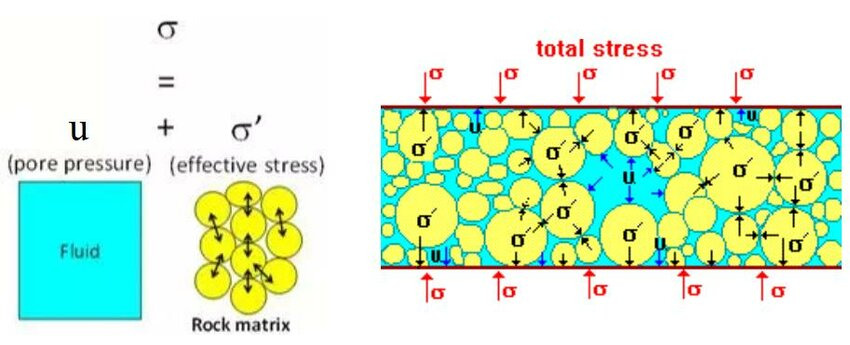
\includegraphics[width=10cm,height=6cm,keepaspectratio]{.//Pics//porepressure.png}
%    \caption{Diagram illustrating the effective stress principle in a saturated cohesionless soil \cite{phdthesis}}
%    \end{figure}
%\end{frame}
%\begin{frame}{Evolución de presión de poros}
%    Se usa una ecuación de advección con relajación:
%    \begin{align}
%    {\partial p \over \partial t} + u\cdot \nabla p = \frac{p_{eq}(h,C,\|u\|)-p}{\tau_p}
%    \end{align}
%    Un ejemplo simple para equilibrio de presión:
%    \begin{align}
%        p_{eq}=\chi_p\rho_m gh\phi(C)\frac{\|u\|}{\|u\|+u_*}, && \phi(C)=\frac{C}{C+C_*}
%    \end{align}
%    que aumenta con espesor y con concentración, y satura con velocidad. Esto captura cualitativamente el aumento de presión por mezcla densa y cizalle.
% 
%\end{frame}

%/////////////////////////////////////////////%
%/////////////////////////////////////////////%

%\subsection{Red neuronal como aproximador}
%\begin{frame}{Arquitectura}
%    \begin{itemize}
%        \item La arquitectura de la red neuronal es un MLP (Multi-Layer Perceptron) con cinco capas ocultas, cada una con 192 neuronas.
%        \item Cada capa oculta utiliza la función de activación $swish$.
%        \item Variables de entrada: $h, C, p, z_b\, (Variable futura)$ 
%    \end{itemize}
%\end{frame}

%\begin{frame}{Condiciones iniciales y fronteras}
%    \begin{itemize}
%        \item Ansatz IC Crater
%        \item BC Dirichlet y Neumann
%    \end{itemize}
%\end{frame}

%\begin{frame}{Variantes}
%    \begin{itemize}
%        \item Rahaman Spectral Bias
%        \item $z_b$ como variable de entrada
%        \item curriculum learning
%    \end{itemize}
%\end{frame}
%
%\begin{frame}{trabajos futuros}
%    \begin{itemize}
%        \item Lambda adaptativo
%        \item seqtoseq
%    \end{itemize}
%\end{frame}


%/////////////////////////////////////////////%
%/////////////////////////////////////////////%


\section{Topografía}
\begin{frame}{DEM ALOS PALSAR 12.5M}
    \begin{figure}
        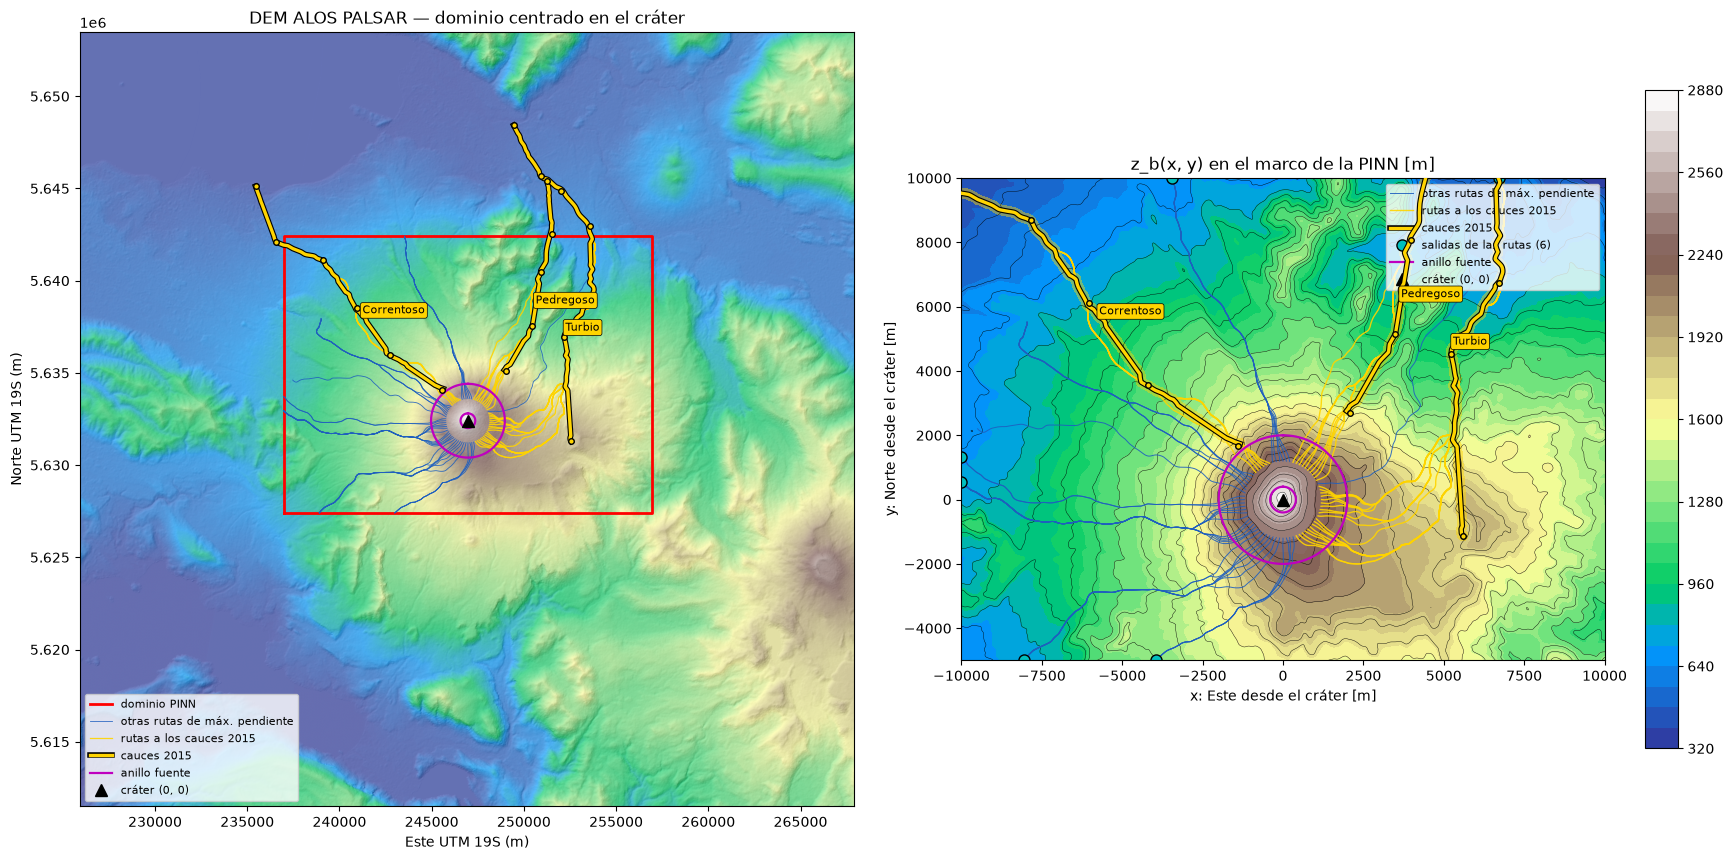
\includegraphics[width=12cm]{Pics/DEMALOSPres.png}
        \caption{Digital Elevation Model (DEM) ALOS PALSAR 12.5M del Volcán Villarrica}
    \end{figure}
\end{frame}



%/////////////////////////////////////////////%
%/////////////////////////////////////////////%



\begin{frame}[allowframebreaks]{Referencias}
    \tiny
    % Esto cambia el ícono de documento por los números [1], [2] del estilo IEEE
    \setbeamertemplate{bibliography item}[text] 
    
    \nocite{*} % Muestra todas las referencias de tu archivo BibTesis.bib
    \bibliographystyle{ieeetr}
    \bibliography{BibTesis} % Asegúrate de que tu archivo se llame BibTesis.bib
\end{frame}

\end{document}